\documentclass{article} % For LaTeX2e
\usepackage{iclr2026_conference,times}

\usepackage{amsmath,amssymb,amsthm}
\usepackage{graphicx}
\usepackage{booktabs}
\usepackage{multirow}
\usepackage{hyperref}
\usepackage{url}
\usepackage{xcolor}

\newtheorem{proposition}{Proposition}
\newtheorem{lemma}{Lemma}
\newtheorem{definition}{Definition}

\newcommand{\ctxcount}{\textsf{ctx-count}}
\newcommand{\ctxbayes}{\textsf{context-Bayes}}
\newcommand{\idealalpha}{\textsf{ideal-$\alpha$}}
\newcommand{\Wstar}{W^{\star}}
\newcommand{\Vsig}{V_{\mathrm{sig}}}
\newcommand{\nnoise}{n_{\mathrm{noise}}}
\newcommand{\WQK}{W_{QK}}
\newcommand{\WOV}{W_{OV}}

\iclrfinalcopy % Draft: shows author names. REMOVE (or comment) for anonymous submission.

\title{In-Context Learning of Markov Chains under Noise:\\
Circuit Formation, a Sharp Phase Transition, and the\\
Feed-Forward Layer as a Finite-Sample Bayesian Calibrator}

\author{Ashutosh Patidar \& Harish G.\ Ramaswamy\\
Department of Data Science and Artificial Intelligence\\
Indian Institute of Technology Madras\\
Chennai 600036, India\\
\texttt{\{ashutosh.patidar,hariguru\}@dsai.iitm.ac.in}
}

\begin{document}

\maketitle

\begin{abstract}
We study in-context learning (ICL) of Markov chains corrupted by noise in a minimal,
fully transparent two-layer transformer. Every sequence carries its \emph{own} random
transition table (each of ten signal states has two equiprobable successors), and a
density parameter $\alpha$ mixes Markov emissions with tokens from a disjoint noise
sub-vocabulary that leaves the latent state unchanged. The task admits an exact
hierarchy of reference predictors---the oracle floor \idealalpha{}, the posterior
predictive \ctxbayes{}, and the empirical-frequency predictor \ctxcount{}---against
which we measure gradient-descent (GD) solutions \emph{and} exactly hand-constructed
induction circuits, weight for weight. We report four findings. (i) Attention-only
softmax models are functionally a temperature-calibrated count reader: they match a
tuned hand-built induction circuit within $0.05$--$0.09$ nats of KL, and their
residual gap to \ctxcount{} is a pure \emph{calibration} deficit of the softmax
readout. (ii) Circuit formation undergoes a sharp noise-driven phase transition: the
noise-skipping circuit that recovers the state after a noise token forms reliably for
$\alpha\le 0.7$ (post-noise wrong-successor rate ${\sim}0.3\%$) but fails to form for
$\alpha\ge 0.8$ (${\sim}50\%$) across a seven-seed sweep; adding a feed-forward layer
restores formation, sometimes through long multi-stage plateaus. (iii) The
feed-forward layer's function is \emph{finite-sample Bayesian calibration}: a hand-set
GELU construction that equalises observed successors toward the \ctxbayes{} target
matches trained FFN models within $\pm0.015$ nats across all $\alpha$, and we prove
the FFN's advantage vanishes with infinite context and under unstructured (Dirichlet)
transition priors---a prediction confirmed on an unequal-successor variant of the
task. (iv) Re-parametrising attention by the gauge-free products
$(\WQK,\WOV)$ improves identifiability but trains markedly slower, consistent with
the implicit acceleration of over-parametrised factorisations; gauge-aware comparison
shows GD reproduces the hand construction's second-layer induction and copy circuits
up to gauge (cosine $0.77$--$0.97$) while realising the first layer differently.
Together these results give a mechanistic, construction-grounded account of what
gradient descent finds---and when it fails---in statistical induction heads under noise.
\end{abstract}

\section{Introduction}
\label{sec:intro}

In-context learning (ICL)---the ability of a trained sequence model to infer a rule
from its prompt and apply it to new queries without weight updates---is arguably the
defining capability of modern transformers \citep{brown2020language}. A now-standard
strategy for understanding ICL mechanistically is to shrink the setting until every
moving part is visible: small transformers, synthetic data whose generative process is
controlled exactly, and hand-constructed reference circuits
\citep{elhage2021mathematical,olsson2022context,bietti2023birth,reddy2024mechanistic}.
For data drawn from random Markov chains, this program has established that two-layer
attention models learn \emph{statistical induction heads} that estimate in-context
bigram statistics \citep{edelman2024evolution,akyurek2024incontext}, characterised the
loss landscape and its unigram traps
\citep{makkuva2024attention,makkuva2024local,varre2025learning}, and proved that
two layers suffice to represent induction heads for any-order chains
\citep{rajaraman2024transformers,ekbote2025what}.

Almost all of this work, however, studies \emph{clean} Markov data, and almost none of
it asks the identifiability question at the level of weights: does GD converge to the
circuit we can construct by hand, or merely to something functionally similar in a
different gauge? This paper addresses both gaps with a single controlled benchmark.
Our task corrupts per-sequence random Markov chains with a disjoint \emph{noise
sub-vocabulary}: with probability $\alpha$ the next token follows the in-context
transition table (and the latent state advances), and with probability $1-\alpha$ a
uniform noise token is emitted (the state is unchanged). The noise density $1-\alpha$
is a continuous difficulty knob that leaves the optimal predictor analytically
tractable: we derive the exact oracle floor (\idealalpha{}), the Bayes-optimal
context-measurable predictor (\ctxbayes{}), and the empirical-frequency predictor
(\ctxcount{}), and we hand-construct a two-layer induction circuit $\Wstar$ that
computes in-context successor frequencies exactly. Every trained model is then
measured against this ladder---in cross-entropy, in KL divergence, in behavioural
diagnostics, and (after quotienting the attention gauge) in weight space.

\textbf{Contributions.} On this benchmark we establish:
\begin{enumerate}
\item \textbf{A transparent testbed with an exact predictor hierarchy}
(\S\ref{sec:task}). The disentangled architecture keeps every residual-stream
coordinate interpretable, and the hierarchy
$\idealalpha \le \ctxbayes \le \ctxcount$ (Proposition~\ref{prop:hierarchy}) turns
cross-entropy plots into readable statements about \emph{which computation} a model
has learned. A closed-form argmax ceiling $\max(\alpha/2,(1-\alpha)/\nnoise)$
calibrates every accuracy number.
\item \textbf{What attention-only GD finds} (\S\ref{sec:gd}). Trained softmax
attention models implement the induction circuit but read it out at a learned
temperature: they sit within $0.05$--$0.09$ nats KL of the tuned hand construction,
while a fixed calibration gap of $0.10$--$0.28$ nats separates them from \ctxcount{}.
Gauge-aware structural comparison shows the second-layer induction and copy circuits
match $\Wstar$ up to gauge (cosine $0.77$--$0.97$), whereas the first-layer
previous-token matcher is realised by a genuinely different solution (cosine
${\approx}\,0$).
\item \textbf{A sharp noise-driven phase transition in circuit formation}
(\S\ref{sec:phase}). Predicting immediately after a noise token requires a
noise-skipping circuit that recovers the state from the last signal token. For
attention-only models this circuit forms for $\alpha\le0.7$ (post-noise
wrong-successor rate ${\sim}0.3\%$) and fails for $\alpha\ge0.8$ (${\sim}50\%$),
robustly across seven seeds; the incentive to build it scales with the noise density
$1-\alpha$. One feed-forward layer restores formation---immediately in some runs,
after staged plateaus reminiscent of grokking in others.
\item \textbf{The feed-forward layer is a finite-sample Bayesian calibrator}
(\S\ref{sec:ffn}). A ladder of hand-set readouts on the \emph{same} frozen attention
shows exactly what each ingredient buys: temperature tuning ($1.85\to1.85$ nats at
$\alpha{=}0.8$), a $\log(\mathrm{count}+\beta)$ FFN ($\to1.60$), and a GELU
``equalize'' step targeting \ctxbayes{} ($\to1.57$)---matching, and at three
densities beating, the GD-trained FFN model, within $\pm0.015$ nats of it everywhere.
We prove the FFN's gain over \ctxcount{} is a finite-sample effect that (a) vanishes
as context length grows (Proposition~\ref{prop:infinite}) and (b) vanishes for
unstructured Dirichlet transition priors by conjugacy
(Proposition~\ref{prop:dirichlet}); an unequal-successor variant of the benchmark
confirms the prediction empirically.
\item \textbf{Identifiability versus trainability of the attention parametrisation}
(\S\ref{sec:gauge}). Attention depends on its weights only through
$\WQK=W_Q^{\top}W_K$ and $\WOV=W_OW_V$; training in the collapsed coordinates removes
the within-head $\mathrm{GL}(d)$ gauge (we verify the collapse of $\Wstar$ is exact,
$\max|\Delta|=0$) but converges markedly slower and to worse solutions at equal
budget, consistent with the implicit acceleration of over-parametrised matrix
factorisation \citep{arora2018optimization,kobayashi2024weight}.
\end{enumerate}

Novel relative to prior Markov-ICL work are (a) the explicit noise sub-vocabulary
with a swept density and the phase transition it induces, (b) the gauge-aware,
weight-level comparison between GD solutions and an exact construction, and (c) the
characterisation of the feed-forward layer as a finite-sample Bayesian calibrator
with provable no-gain regimes. Concurrently and independently,
\citet{agarwal2025bayesian} report that in controlled Bayesian tasks the feed-forward
network performs the posterior update while attention routes evidence---consistent
with, and complementary to, our construction-level account.

\section{Related work}
\label{sec:related}

\textbf{Induction heads and Markov ICL.} Induction heads were identified as the core
ICL circuit by \citet{elhage2021mathematical} and \citet{olsson2022context}.
\citet{edelman2024evolution} introduced ICL of per-sequence random Markov chains and
observed statistical induction heads forming through simpler-to-complex stages;
\citet{bietti2023birth} and \citet{reddy2024mechanistic} analysed the abruptness of
induction-head emergence; \citet{akyurek2024incontext} benchmarked architectures on
in-context language learning. The Makkuva line characterised loss landscapes and
learning dynamics of transformers on Markov data
\citep{makkuva2024attention,makkuva2024local}, culminating in representation results
for any-order chains \citep{rajaraman2024transformers,ekbote2025what}.
\citet{nichani2024transformers} proved GD learns causal structure in related settings,
\citet{chen2024unveiling} proved formation of generalised induction heads with an
explicit FFN role, and \citet{wang2024how} gave approximation and dynamics analyses.
\citet{dangelo2025selective} study selection among competing lags interleaved in one
sequence. Our benchmark differs from all of these in corrupting the chain with a
disjoint, density-swept noise sub-vocabulary while keeping the Bayes-optimal
predictors in closed form.

\textbf{Phase transitions and plateaus in circuit formation.}
Data-distributional control of induction-circuit emergence is an active frontier:
\citet{zucchet2025emergence} derive emergence-time scalings and a signal-dilution
mechanism; \citet{kawata2025shortcut} prove a diversity-controlled transition between
induction heads and positional shortcuts; \citet{lavie2026phase} obtain a first-order
phase transition for copy-subcircuit formation; \citet{varre2025learning} show
sub-$n$-gram solutions are near-stationary points, explaining stage-wise plateaus;
\citet{singh2024what} dissect the co-adapting subcircuits behind abrupt formation;
\citet{musat2025emergence} reduce emergence dynamics to a few parameters. Our
transition differs in its control knob---noise density, holding task diversity,
vocabulary, and length fixed---and in coming with an exact accounting of the CE that
the missing circuit costs.

\textbf{ICL as Bayesian inference and the role of the FFN.} Bayesian accounts of ICL
range from posterior-predictive theory \citep{wakayama2025incontext} to empirical
near-optimality on HMMs \citep{dai2025pretrained}. Closest to our \S\ref{sec:ffn},
\citet{agarwal2025bayesian} localise the posterior update in the FFN in controlled
``wind-tunnel'' tasks, and \citet{sun2025role} prove FFN layers enable nonlinear ICL
that attention alone cannot express; \citet{smart2025incontext} show one attention
layer can realise Bayes-optimal denoising for Gaussian priors. We add the
construction-level mechanism (log-domain readout plus prior-dependent equalisation)
and the two no-gain regimes, which sharpen \emph{when} an FFN can pay at all.

\textbf{Parametrisation, gauge, and implicit bias.} That attention depends only on
$\WQK$ and $\WOV$ is classical \citep{elhage2021mathematical}; the induced parameter
symmetries have been formalised as gauge invariances \citep{vannierop2024transformer}.
\citet{arora2018optimization} showed over-parametrised factorisation acts as a
preconditioner (implicit acceleration), and \citet{kobayashi2024weight} that weight
decay biases attention factor products toward low rank. We connect these threads
empirically: the gauge-free parametrisation is more identifiable yet slower to train,
an explicit identifiability--trainability trade-off.

\section{The noisy Markov ICL task and its exact reference predictors}
\label{sec:task}

\begin{figure}[t]
\centering
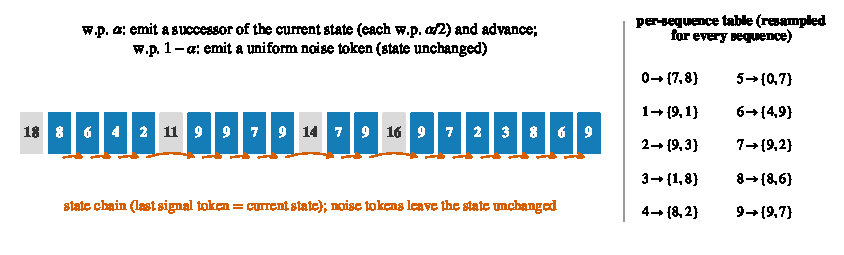
\includegraphics[width=\textwidth]{figures/fig_task.pdf}
\caption{\textbf{The noisy Markov ICL task.} Each sequence draws its own transition
table over the $\Vsig=10$ signal tokens (right); every signal state has exactly two
equiprobable successors. At each step, with probability $\alpha$ a successor of the
current state is emitted (blue; the state advances along the orange chain), and with
probability $1-\alpha$ a uniform token from the disjoint noise sub-vocabulary is
emitted (grey; the state is unchanged). The model must infer the table from context;
loss is evaluated on the last $100$ of $T=200$ positions.}
\label{fig:task}
\end{figure}

\textbf{Generative process.} The vocabulary has $V=20$ tokens: signal tokens
$\{0,\dots,9\}$ ($\Vsig=10$) and noise tokens $\{10,\dots,19\}$ ($\nnoise=10$). For
each sequence independently, every signal state $s$ draws an unordered pair of
distinct successors $\{\sigma_1(s),\sigma_2(s)\}$ uniformly at random. Generation
tracks a latent state (the last emitted signal token): with probability $\alpha$ the
next token is $\sigma_1$ or $\sigma_2$ of the current state (probability $\alpha/2$
each) and becomes the new state; with probability $1-\alpha$ the next token is uniform
on the noise sub-vocabulary and the state is unchanged (Figure~\ref{fig:task}).
Sequences have length $T=200$; loss and all evaluations use the final $100$ positions,
so the model always has substantial context. We sweep
$\alpha\in\{0.1,\dots,0.9\}$; per $\alpha$ we train on $20{,}000$ sequences and
checkpoint by held-out CE, and \emph{all numbers reported in this paper are computed
on $5{,}000$ freshly generated evaluation sequences} never used for training or model
selection (Appendix~\ref{app:setup}).

\textbf{Architecture.} We use a \emph{disentangled} transformer
\citep{elhage2021mathematical,edelman2024evolution}: the input is the concatenation of
a one-hot token encoding and a one-hot position encoding ($D_0=V+T=220$), and each of
two causal attention blocks \emph{concatenates} its output onto the residual stream,
$s \mapsto [\,s,\ \mathrm{attn}(s)\,]$, so layer widths grow $220\to440\to660$ and
every coordinate retains a fixed, interpretable meaning. A linear unembedding (with
bias) produces logits. Attention blocks use single-head softmax attention with
separate $W_Q,W_K,W_V,W_O$ (attention width $220$). Variants add one position-wise
GELU FFN before the unembedding (\emph{+FFN}; hidden width $128$), an FFN after each
attention block (\emph{two-cell}), and/or replace $(W_Q,W_K,W_V,W_O)$ by the combined
matrices $(\WQK,\WOV)$ (\S\ref{sec:gauge}). No LayerNorm is used, keeping all
circuits linear-algebraically transparent. Training details are in
Appendix~\ref{app:setup}.

\subsection{The exact predictor hierarchy}
\label{sec:hierarchy}

Three reference predictors anchor every comparison. Write $c(s,\cdot)$ for the
empirical successor counts of state $s$ accumulated over the context (each signal
token following state $s$, possibly across intervening noise, increments one count),
$n(s)=\sum_k c(s,k)$, and let the \emph{query state} at position $t$ be $x_t$ if
$x_t$ is a signal token, else the last signal token before $t$.

\begin{definition}[Reference predictors]\label{def:refs}
For query state $s$ with counts $c=c(s,\cdot)$ and $n=n(s)$:
\emph{(a)} \idealalpha{} knows the true pair and puts $\alpha/2$ on each true
successor and $(1-\alpha)/\nnoise$ on each noise token.
\emph{(b)} \ctxcount{} puts $\alpha\,(c_k+\epsilon)/\sum_j(c_j+\epsilon)$ on signal
token $k$ (add-$\epsilon$ smoothing, $\epsilon=0.01$) and $(1-\alpha)/\nnoise$ on
noise.
\emph{(c)} \ctxbayes{} is the exact posterior predictive under the generative prior:
with $m=|\{k: c_k>0\}|$ observed distinct successors, it puts $\alpha/2$ on each
observed successor and splits the remaining successor mass uniformly over the
$\Vsig-m$ unobserved signal tokens when $m\le 1$ (Appendix~\ref{app:bayes}); noise
mass is exact.
\end{definition}

\begin{proposition}[Hierarchy]\label{prop:hierarchy}
In expectation over the generative process,
$\mathrm{CE}(\idealalpha) \le \mathrm{CE}(\ctxbayes) \le \mathrm{CE}(\ctxcount)$,
and \ctxbayes{} is optimal among all predictors measurable with respect to the
context. (Proof: Appendix~\ref{app:proofs}.)
\end{proposition}

\begin{lemma}[Argmax ceiling]\label{lem:ceiling}
Any next-token predictor's accuracy is at most
$\max\!\big(\alpha/2,\ (1-\alpha)/\nnoise\big)$, the accuracy of the oracle argmax.
For $\alpha\ge 1/6$ this equals $\alpha/2$; e.g.\ $0.40$ at $\alpha=0.8$.
\end{lemma}

The hierarchy is tight and informative: on fresh data at $\alpha=0.8$ the three
levels are $1.5125$, $1.5268$, and $1.5697$ nats. The $\ctxbayes$--$\ctxcount$ gap
($0.043$ nats here) is the \emph{entire} headroom that any nonlinearity beyond count
normalisation can win from a finite context, a fact \S\ref{sec:ffn} exploits; the
$\idealalpha$--$\ctxbayes$ gap is unreachable by any context-only predictor.

\subsection{An exact hand-constructed induction circuit}
\label{sec:wstar}

Following the induction-head recipe \citep{elhage2021mathematical}, we hand-set the
weights of the two-layer disentangled architecture into a
\emph{PerfectInductionTransformer} $\Wstar$: layer~1 attends each position to its
predecessor via the position--position block of $W_{QK}^{(1)}$ (a $-20(t_q-t_k)$
ramp with the diagonal masked) and copies the predecessor's token identity; layer~2
attends from the current query state to every position whose \emph{predecessor}
carried that state, restricted to signal tokens, and averages their one-hot
successors. The attention output at the readout coordinates is then exactly the
normalised empirical successor-frequency vector $f(s)=c(s,\cdot)/n(s)$, and the
unembedding selects it. Full weight matrices are in Appendix~\ref{app:wstar}.
$\Wstar$ is both a constructive expressivity proof for this architecture and the
reference point for all weight-space comparisons. Its one deficiency is deliberate:
a \emph{linear} readout of $f$ passed through the final softmax re-exponentiates the
frequencies, so even the best global temperature $\sigma$ leaves a large CE gap
(Figure~\ref{fig:ffn}); making this precise---and repairing it---is the subject of
\S\ref{sec:ffn}.

\section{What attention-only gradient descent finds}
\label{sec:gd}

\begin{figure}[t]
\centering
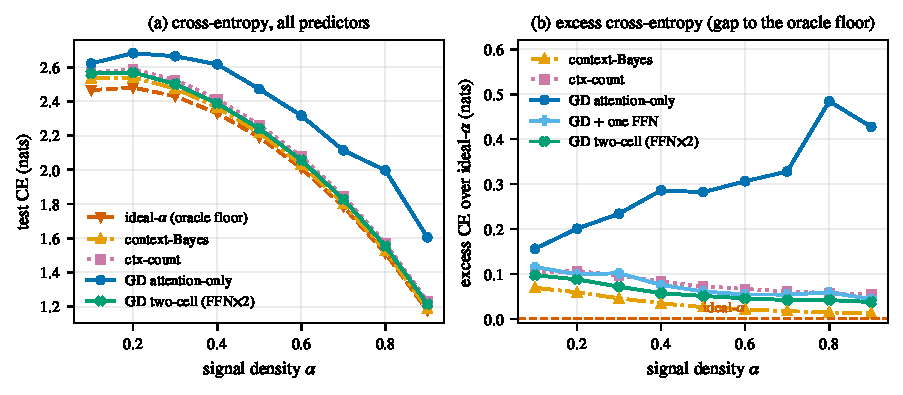
\includegraphics[width=\textwidth]{figures/fig_hierarchy.pdf}
\caption{\textbf{The predictor hierarchy and trained models} (fresh evaluation data,
$5{,}000$ sequences per $\alpha$; CE on positions $100$--$200$).
\textbf{(a)} absolute cross-entropy; \textbf{(b)} excess CE over the oracle floor
\idealalpha{}. FFN-augmented models (GD + one FFN, two-cell) track \ctxcount{} and
push below it toward \ctxbayes{} at high $\alpha$; the attention-only model carries
an additional calibration gap that spikes at the $\alpha=0.8$ phase transition
(\S\ref{sec:phase}).}
\label{fig:hierarchy}
\end{figure}

Figure~\ref{fig:hierarchy} places GD-trained models on the hierarchy (all
cross-entropies are tabulated in Table~\ref{tab:full-ce}; per-position diagnostics in
Appendix~\ref{app:figs}). Three observations organise everything that follows.

\textbf{(1) FFN-augmented models sit on \ctxcount{}---and beyond.} The two-cell model
matches \ctxcount{} at low $\alpha$ and \emph{beats} it for $\alpha\ge0.4$ (e.g.\
$1.5541$ vs.\ $1.5697$ at $\alpha=0.8$), moving toward the \ctxbayes{} optimum
($1.5268$): the trained FFN is exploiting the two-equiprobable-successor prior, not
merely normalising counts. The single-FFN model behaves identically to within a few
millinats.

\textbf{(2) Attention-only models are temperature-calibrated count readers.} The
attention-only softmax model tracks the \emph{shape} of the hierarchy but with a
$0.10$--$0.28$ nat offset. Functionally it is far closer to the tuned hand
construction than to \ctxcount{}: per-position KL from the trained model to
$\Wstar$ with per-$\alpha$ tuned temperature and noise bias is $0.05$--$0.09$ nats
for $\alpha\le0.7$, versus $0.19$--$0.33$ nats to \ctxcount{}
(Table~\ref{tab:kl-cos}, left). In other words, GD finds the induction circuit and
the best \emph{linear-readout} calibration of it, and the remaining offset is exactly
what a linear readout cannot fix (Proposition~\ref{prop:noaffine}).

\textbf{(3) Up to gauge, layer 2 matches the construction; layer 1 does not.}
Attention depends on its weights only through the products
$\WQK=W_Q^\top W_K$ and $\WOV=W_OW_V$, so raw weight comparisons are meaningless;
we compare gauge-invariant products, folded into the interpretable input coordinates
(Appendix~\ref{app:gauge}). The trained models' layer-2 \emph{induction match}
circuit (query-state $\to$ predecessor-token block) and \emph{copy} circuit
($\WOV^{(2)}$ into the unembedding) align with $\Wstar$'s at cosine $0.77$--$0.93$
and $0.95$--$0.97$ respectively across all $\alpha$; the layer-1 previous-token
matcher aligns at cosine ${\approx}\,0$ (Table~\ref{tab:kl-cos}, right). Behavioural
probes agree: trained layer-1 attention peaks at offset~$1$ and layer-2 induction
mass is $0.73$ (vs.\ $0.80$ for $\Wstar$). GD thus reproduces the second-layer
circuit essentially up to gauge and temperature, while solving the first-layer
sub-problem with a genuinely different (distributed, position-mixing) realisation
than the crisp $-20(t_q{-}t_k)$ ramp we constructed---an instance of functional
convergence \emph{without} weight-level convergence even after the gauge is
quotiented out.

\begin{table}[t]
\centering
\small
\caption{\textbf{Left:} per-position KL (nats, $N{=}200$ sequences) from the trained
attention-only model to \ctxcount{} and to the temperature-tuned construction
$\Wstar(\sigma,b_N)$; the trained model is a calibrated count reader. \textbf{Right:}
gauge-invariant cosine similarity of trained circuits (combined-parametrisation
models) to $\Wstar$: layer-2 induction-match and copy circuits align; the layer-1
previous-token circuit is realised differently.}
\label{tab:kl-cos}
\begin{tabular}{@{}lcc@{\hspace{2.2em}}cccc@{}}
\toprule
& \multicolumn{2}{c@{\hspace{2.2em}}}{$\mathrm{KL}(\mathrm{GD}\,\|\,\cdot)$}
& \multicolumn{4}{c}{$\cos(\mathrm{GD},\Wstar)$ (gauge-invariant)}\\
\cmidrule(r{2.2em}){2-3}\cmidrule{4-7}
$\alpha$ & \ctxcount & $\Wstar(\sigma,b_N)$ & induction & copy & $\WOV^{(1)}$ & prev-tok \\
\midrule
0.1 & 0.194 & 0.060 & 0.926 & 0.958 & 0.005 & 0.030\\
0.3 & 0.210 & 0.053 & 0.797 & 0.966 & $-$0.002 & 0.092\\
0.5 & 0.277 & 0.064 & 0.850 & 0.947 & $-$0.074 & 0.141\\
0.7 & 0.325 & 0.073 & 0.915 & 0.957 & $-$0.016 & 0.122\\
0.8 & 0.843 & 0.337 & 0.922 & 0.953 & 0.056 & 0.131\\
0.9 & 0.608 & 0.209 & 0.928 & 0.947 & $-$0.033 & 0.140\\
\bottomrule
\end{tabular}
\end{table}

\section{A noise-driven phase transition in circuit formation}
\label{sec:phase}

\begin{figure}[t]
\centering
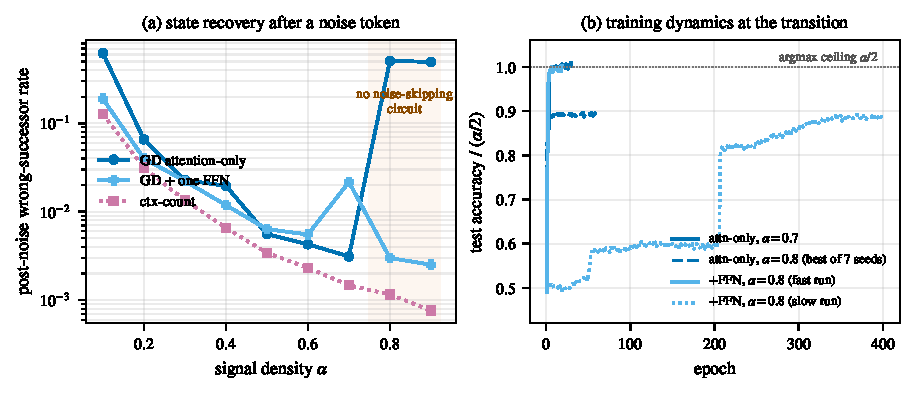
\includegraphics[width=\textwidth]{figures/fig_phase.pdf}
\caption{\textbf{The noise-driven phase transition.} \textbf{(a)} Wrong-successor
rate of the argmax over signal tokens, restricted to positions whose input token is
noise---exactly the positions that require the noise-skipping circuit. The
attention-only model matches the analytic \ctxcount{} argmax for
$0.2\le\alpha\le0.7$ and jumps to ${\sim}50\%$ (successor-pair chance level) for
$\alpha\ge0.8$; one FFN restores formation. \textbf{(b)} Test accuracy normalised by
the argmax ceiling $\alpha/2$ (Lemma~\ref{lem:ceiling}). At $\alpha=0.8$ the
attention-only model plateaus at $0.90$ of its ceiling (best of seven seeds); +FFN
runs reach the ceiling either immediately or through staged plateaus.}
\label{fig:phase}
\end{figure}

The genuinely hard sub-task in this benchmark is hidden in plain sight: predicting
\emph{immediately after a noise token}. There the query must ignore the current
(noise) token, recover the state from the last signal token, and run the induction
lookup from that recovered state---a \emph{noise-skipping} extension of the induction
circuit. We isolate it with a targeted metric: at evaluation positions whose input
token is noise, take the model's argmax over signal tokens and score it against the
true successor pair (chance level for a model that has the induction circuit but
guesses the state is ${\sim}50\%$, since a wrong state's pair almost never overlaps
the true pair by more than luck).

\textbf{A sharp transition at $\alpha\approx0.8$.} Figure~\ref{fig:phase}(a) shows
the post-noise wrong-successor rate. For $0.2\le\alpha\le0.7$ the attention-only
model is essentially perfect ($0.3$--$6.6\%$, tracking the analytic \ctxcount{}
argmax); at $\alpha=0.8$ it jumps to $50.7\%$ and at $\alpha=0.9$ to $49.6\%$: the
noise-skipping circuit simply did not form. The CE cost is visible as the
$\alpha=0.8$ spike in Figure~\ref{fig:hierarchy}(b) ($+0.43$ nats over \ctxcount{};
full rate tables in Table~\ref{tab:postnoise}).
This is not a seed accident: a seven-seed sweep with a probe-and-abandon protocol
left every seed at test accuracy $0.359$ against a ceiling of $0.40$
(Figure~\ref{fig:phase}(b)); nor is it a data or width artefact (regenerated data
and wider models reproduce it; Appendix~\ref{app:setup}).

\textbf{Why noise density controls formation.} The fraction of loss positions that
exercise the noise-skipping circuit is exactly the noise density $1-\alpha$. For
$\alpha\le0.7$, at least $30\%$ of the training signal rewards building it; at
$\alpha=0.8$ only $20\%$ does, while the remaining $80\%$ of positions are already
served by the plain induction circuit---so the gradient toward the harder circuit is
both smaller and swamped by the variance of the easy positions. The asymmetric
outcome (formation at high noise, failure at low-but-nonzero noise) makes
$\alpha\approx0.8$ the worst case: past the transition yet still paying $20\%$ of
positions at chance. This is a data-distributional formation threshold in the spirit
of the diversity transition of \citet{kawata2025shortcut} and the signal-dilution
account of \citet{zucchet2025emergence}, with noise density as the control parameter
and an exact accounting (via the hierarchy) of what the missing circuit costs; the
near-stationarity of partial solutions \citep{varre2025learning,makkuva2024local}
offers a consistent landscape-level interpretation of the stuck plateau.

\textbf{The FFN changes the transition.} With one FFN the circuit forms at every
$\alpha$: the post-noise rate at $\alpha\ge0.8$ drops to $0.3\%$. Formation is not
always immediate---Figure~\ref{fig:phase}(b) shows one $\alpha=0.8$ run reaching the
ceiling within ${\sim}5$ epochs and another crawling through two long plateaus
(epochs ${\sim}20$--$60$ and ${\sim}70$--$270$) before climbing, the staged pattern
familiar from sequential-learning analyses
\citep{edelman2024evolution,varre2025learning,singh2024what}. We read this as the
FFN both smoothing the loss landscape around the count-reading solution and
decoupling calibration from circuit formation: with the readout repaired by the FFN
(\S\ref{sec:ffn}), the marginal value of the noise-skipping circuit is a larger
share of the remaining loss.

\section{The feed-forward layer is a finite-sample Bayesian calibrator}
\label{sec:ffn}

\begin{figure}[t]
\centering
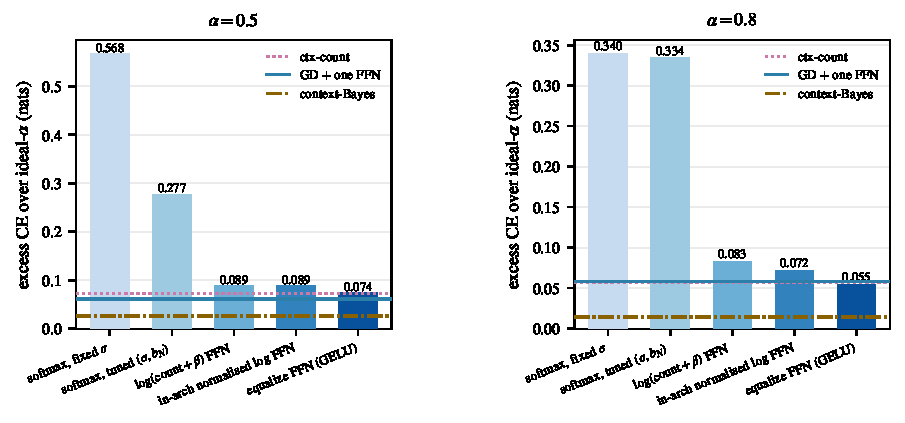
\includegraphics[width=\textwidth]{figures/fig_ffn.pdf}
\caption{\textbf{The calibration ladder}: excess CE over \idealalpha{} of five
hand-set readouts on the \emph{same} frozen $\Wstar$ attention (bars), against the
analytic references and the GD-trained single-FFN model (lines). A softmax readout of
the count vector is poorly calibrated at any temperature; a
$\log(\mathrm{count}+\beta)$ FFN recovers \ctxcount{}; the GELU equalize FFN targets
\ctxbayes{} and matches the trained model.}
\label{fig:ffn}
\end{figure}

Why does one small FFN turn a $0.28$-nat calibration gap into a predictor that beats
\ctxcount{}? This section answers constructively, by hand-setting a ladder of
readouts on the \emph{same} frozen $\Wstar$ attention and measuring each rung
(Figure~\ref{fig:ffn}).

\textbf{The problem: softmax re-exponentiates counts.} $\Wstar$'s attention output
is the frequency vector $f(s)$. A linear unembedding feeds $\sigma f$ to the softmax,
which outputs $\propto e^{\sigma f_k}$---an exponential distortion of the very
quantity the circuit computed. No temperature or bias repairs this:

\begin{proposition}[No affine readout suffices]\label{prop:noaffine}
There is no temperature $\sigma$ and bias $b$ for which
$\mathrm{softmax}(\sigma f + b)$ equals the \ctxcount{} distribution for all count
vectors; the required correction depends on the instance through $\log f$.
(Appendix~\ref{app:proofs}.)
\end{proposition}

Empirically the best fixed-$\sigma$ readout sits $0.34$ nats above \idealalpha{} at
$\alpha=0.8$ and per-$\alpha$ tuning of $(\sigma,b_N)$ barely helps ($0.334$)---the
same level as the trained attention-only model, corroborating \S\ref{sec:gd}(2).

\textbf{Rung 1: a log-domain FFN recovers \ctxcount{}.} Because
$\mathrm{softmax}(\log p)=p$, an FFN that maps the count coordinates through
$z_k=\log(f_k+\beta)$ (with separate floors for signal and noise coordinates) makes
the softmax output the floored, normalised counts exactly. A piecewise-linear
realisation with six GELU hinges---the model's own activation---implements it inside
the architecture (weights in Appendix~\ref{app:constructions}) and lands within
$0.02$--$0.03$ nats of \ctxcount{} at every $\alpha$ ($0.083$ vs.\ $0.057$ excess at
$\alpha=0.8$); a strictly in-architecture normalised variant is similar ($0.072$).

\textbf{Rung 2: an equalize FFN reaches the trained model.} The remaining
headroom---\ctxcount{} to \ctxbayes{}---comes from the \emph{prior}: with two
equiprobable successors, the Bayes rule ignores the observed ratio $c_1\!:\!c_2$ and
assigns $\alpha/2$ to each observed successor (Definition~\ref{def:refs}). A single
GELU soft-step per signal coordinate implements exactly this: observed successor
$\mapsto \log(\alpha/2)$, unobserved signal $\mapsto$ a tuned floor, noise coordinate
$\mapsto$ the exact constant $\log((1-\alpha)/\nnoise)$. This \emph{equalize}
construction---three interpretable parameters per density, set once offline
(Appendix~\ref{app:constructions})---matches the GD-trained FFN model within
$\pm0.015$ nats at every $\alpha$ and beats it at $\alpha\in\{0.1,0.3,0.8\}$ (e.g.\
$1.5672$ vs.\ $1.5711$ at $\alpha=0.8$). We conclude that what the trained FFN
computes is, to within measurement precision, \emph{log-domain count reading plus
prior-driven equalisation}: a finite-sample Bayesian calibration head. Ablations
agree: in the two-cell model, linearising or removing either FFN sharply raises CE,
with the last FFN dominating final calibration.

\textbf{When can an FFN help at all?} Two propositions bound the mechanism's scope.

\begin{proposition}[The gain is finite-sample]\label{prop:infinite}
As the number $n$ of in-context observations of the queried state grows, both
\ctxcount{} and \ctxbayes{} converge to \idealalpha{}, and the FFN-attainable gain
$\mathrm{CE}(\ctxcount)-\mathrm{CE}(\ctxbayes)$ decays as $O(1/n)$.
(Appendix~\ref{app:proofs}.)
\end{proposition}

\begin{proposition}[No gain without structure]\label{prop:dirichlet}
If instead each transition row is drawn from a Dirichlet$(\beta)$ prior over all
$\Vsig$ signal tokens, the exact posterior predictive \emph{is} add-$\beta$-smoothed
\ctxcount{} (Dirichlet--multinomial conjugacy). Count normalisation is then already
Bayes-optimal among context-measurable predictors, and no readout---FFN or
otherwise---can improve on it. (Appendix~\ref{app:proofs}.)
\end{proposition}

The FFN's value on this benchmark thus exists precisely because the successor prior
is \emph{structured} (sparse and equiprobable), and only at \emph{finite} context.
Both predictions are testable. First, the measured
$\ctxcount{}-\ctxbayes{}$ gap indeed shrinks with effective sample size (it is
$0.043$ nats at $\alpha=0.8$, where each state averages ${\sim}8$ observations in
$100$ context positions, and $0.034$ at $\alpha=0.1$). Second, we re-ran the full
pipeline on a variant benchmark whose successor probabilities are \emph{not}
equiprobable ($p_1\sim U(0,1)$, $p_2=1-p_1$ per state)---a prior under which
equalisation is provably harmful and the count \emph{ratio} must be read out. There,
the trained FFN model lands within $\pm0.02$ nats of the in-architecture
count-normalisation construction at every $\alpha$ (and a Hessian probe places the
construction at a local minimum of the training loss); the equal-split calibration
that wins on the main benchmark loses by up to $0.2$ nats
(Appendix~\ref{app:altered}). The FFN, in short, learns \emph{the calibration the
prior calls for}---equalisation when the prior is equiprobable, ratio read-out when
it is not---and cannot beat plain counting when the prior is unstructured.

\section{Identifiability versus trainability of the attention parametrisation}
\label{sec:gauge}

\begin{figure}[t]
\centering
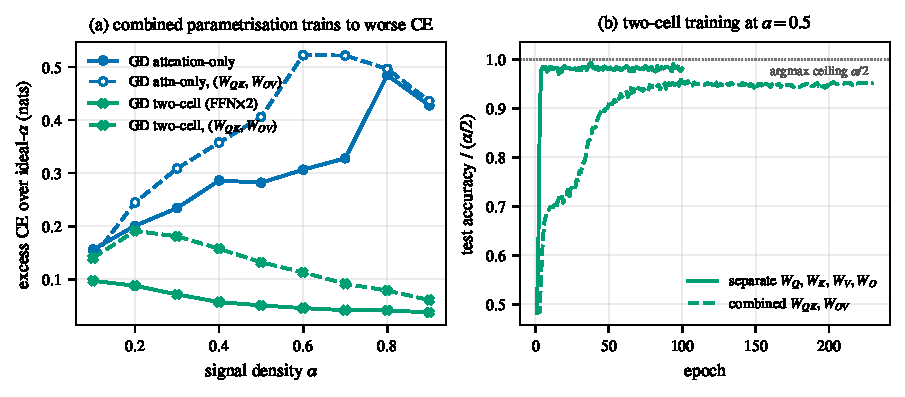
\includegraphics[width=\textwidth]{figures/fig_comb.pdf}
\caption{\textbf{Separate vs.\ combined attention parametrisation.} \textbf{(a)}
Excess CE at equal (or larger) training budget: the combined $(\WQK,\WOV)$ models
(dashed, open markers) are consistently worse than their separately-parametrised
counterparts, for both attention-only and two-cell models. \textbf{(b)} Two-cell
training at $\alpha=0.5$: the separate parametrisation reaches its ceiling in
${\sim}10$ epochs; the combined one crawls for $100{+}$ and saturates lower.}
\label{fig:comb}
\end{figure}

Softmax attention uses its parameters only through $\WQK=W_Q^{\top}W_K$ and
$\WOV=W_OW_V$: the map $(W_Q,W_K,W_V,W_O)\mapsto(\WQK,\WOV)$ is invariant under the
within-head gauge $(W_Q,W_K)\to(GW_Q, G^{-\top}W_K)$,
$(W_V,W_O)\to(HW_V,W_OH^{-1})$ for invertible $G,H$
\citep{elhage2021mathematical,vannierop2024transformer}. For a
construction-vs.-learned comparison this gauge is a nuisance---solutions equal up to
gauge look arbitrarily different in raw weights---so we also train directly in the
collapsed coordinates. Collapsing $\Wstar$ itself is exact: the combined-form
construction reproduces the separate-form logits with $\max|\Delta|=0$
(Appendix~\ref{app:gauge}).

The trade-off is stark (Figure~\ref{fig:comb}). At equal or larger epoch budgets the
combined models are uniformly worse in CE---by $0.04$--$0.24$ nats for the
attention-only family and $0.03$--$0.10$ nats for two-cell models---and their
training curves rise far more slowly (at $\alpha=0.5$: ${\sim}10$ epochs to ceiling
for separate, $100{+}$ epochs to a lower plateau for combined). The phenomenon
matches the known implicit bias of over-parametrised factorisation: GD on a product
$W_Q^\top W_K$ preconditions the effective update on $\WQK$ by the factor
covariances---accelerating and low-rank-biasing it
\citep{arora2018optimization,kobayashi2024weight}---and the collapse forfeits exactly
this. Identifiability and trainability pull in opposite directions: the coordinates
in which solutions are comparable are the coordinates in which GD is slow. Our
gauge-aware comparisons (Table~\ref{tab:kl-cos}) therefore train in the fast
parametrisation and \emph{analyse} in the collapsed one.

\section{Discussion, limitations, and outlook}
\label{sec:discussion}

\textbf{Summary.} On a noisy Markov ICL benchmark with an exact predictor hierarchy,
we find that GD-trained attention learns the hand-constructible induction circuit up
to gauge in its second layer (but not its first), that the softmax readout leaves a
calibration gap no affine readout can fix, that one FFN closes the gap by log-domain
count reading plus prior-driven equalisation---a finite-sample Bayesian calibrator
with provable no-gain regimes---and that circuit formation itself undergoes a sharp
noise-density-driven phase transition that the FFN alleviates. The picture that
emerges is compositional: \emph{attention gathers sufficient statistics; the FFN
applies the prior; and each piece can fail or be repaired independently.}

\textbf{Limitations.} Our claims about GD are budget- and scale-relative: ``the
circuit fails to form'' means under our training protocol (seven seeds, fixed
learning rate, ${\le}200$ epochs at the transition), not information-theoretically.
Most densities were trained with a single seed (the $\alpha=0.8$ sweep is the
exception), so per-$\alpha$ CE differences of a few millinats should be read with
care, though every qualitative claim spans multiple densities and model families.
Structural comparisons (Table~\ref{tab:kl-cos}) use $200$ evaluation sequences and
our specific gauge-invariant projections; alternative invariants exist. The
benchmark itself is deliberately minimal---single-head attention, one-hot
disentangled streams, first-order chains, a two-successor prior---and the FFN
result speaks to \emph{readout} calibration, not to FFNs as key--value memories in
large models.

\textbf{Outlook.} Three directions follow directly. (i) \emph{Toward \idealalpha{}}:
the equalize construction cannot spread mass to the unobserved successor when only
one has been seen; an $n$-aware two-stage FFN could, and would quantify the price of
position-wise readouts. (ii) \emph{General chains}: Proposition~\ref{prop:dirichlet}
delineates where FFN gains can exist at all; interpolating between Dirichlet and
structured priors would trace the full gain curve. (iii) \emph{Formation theory}: our
transition invites a Makkuva-style landscape analysis with noise density as the
control parameter---the stuck solution is plausibly a near-stationary partial
circuit in the sense of \citet{varre2025learning}.

\subsubsection*{Reproducibility statement}
All data are synthetic and fully specified (\S\ref{sec:task},
Appendix~\ref{app:setup}); generators use fixed seeds. Every number in the paper is
produced by a single evaluation harness on $5{,}000$ freshly generated sequences
(seed $13423$) disjoint from training and model selection; hand-construction
parameters searched offline are tabulated in Appendix~\ref{app:constructions}
together with their search grids. Code (data generation, training, constructions,
evaluation, and figure scripts) will be released.

\bibliography{refs}
\bibliographystyle{iclr2026_conference}

\clearpage
\appendix

\section{Task, training, and evaluation details}
\label{app:setup}

\textbf{Data.} Vocabulary $V=20$ ($\Vsig=10$ signal, $\nnoise=10$ noise);
$T=200$; per-$\alpha$ datasets of $20{,}000$ train / $3{,}000$ selection sequences
(fixed seeds), $\alpha\in\{0.1,\dots,0.9\}$. Successor pairs are drawn uniformly over
distinct ordered pairs and used unordered with equal emission probability. The state
is defined as the last emitted signal token; the first signal token of a sequence is
drawn uniformly. All losses and metrics use positions $100$--$200$
(\texttt{suffix\_len}=100).

\textbf{Models and training.} Disentangled transformer, $D_0=220$, attention width
$220$, unembedding bias on; single-FFN variant inserts a residual GELU MLP
($660\to128\to660$) before the unembedding; two-cell variants insert one after each
attention block. Optimiser Adam, constant learning rate ($10^{-2}$ attention-only,
$10^{-3}$ FFN variants), batch $256$, up to $120$--$230$ epochs; checkpoint by best
selection-set CE. The $\alpha=0.8$ attention-only sweep used seeds
$\{42,0,7,1,13,123,2024\}$ with a probe-and-abandon protocol (abandon if selection
accuracy $<0.370$ at epoch $60$; ceiling $0.40$); every seed was abandoned or
plateaued at $0.359$. The combined-parametrisation runs use the same protocol with
$(\WQK,\WOV)$ initialised Xavier-uniform.

\textbf{Evaluation.} All reported CE values, wrong-successor rates, and figures use
$5{,}000$ freshly generated sequences per $\alpha$ (generator seed $13423$, disjoint
from all training/selection data) evaluated in one harness; this removes any
selection bias from checkpointing on the fixed selection set. KL and structural
metrics (Table~\ref{tab:kl-cos}) use $200$ sequences. Compute: single A100 per run;
every experiment fits in ${<}12$ GPU-hours.

\section{The context-Bayes posterior predictive}
\label{app:bayes}

Fix a query state $s$ and let $c\in\mathbb{Z}_{\ge0}^{\Vsig}$ be its successor counts
in the context, $n=\sum_k c_k$, $S=\{k:c_k>0\}$, $m=|S|$. Under the generative prior
the successor pair $P=\{i,j\}$ is uniform over unordered pairs and emissions given
$P$ are i.i.d.\ uniform on $P$, so the likelihood of $c$ is $2^{-n}$ for every pair
$P\supseteq S$ and $0$ otherwise. The posterior is therefore uniform on
$\{P : P\supseteq S\}$ and the predictive successor distribution is
$q(k)=\tfrac{1}{2}\Pr[k\in P\,|\,c]$:
\[
q(k)=
\begin{cases}
\tfrac12\,\mathbf{1}[k\in S], & m=2\quad(\text{pair identified}),\\[2pt]
\tfrac12\,\mathbf{1}[k\in S]+\tfrac12\cdot\tfrac{1}{\Vsig-1}\,\mathbf{1}[k\notin S], & m=1,\\[2pt]
\tfrac{1}{\Vsig}, & m=0,
\end{cases}
\]
and the emitted-token predictive is $\alpha\,q(k)$ on signal token $k$ and exactly
$(1-\alpha)/\nnoise$ on each noise token. Note the rule never uses the ratio
$c_1{:}c_2$---only the support---which is what the equalize construction of
\S\ref{sec:ffn} implements with a soft step.

\section{Proofs}
\label{app:proofs}

\textbf{Proposition~\ref{prop:hierarchy}.} Conditional on the context $\mathcal{C}$,
the true emission distribution of the next token is
$p^{*}(\cdot)=\mathbb{E}[p_{\mathrm{emit}}(\cdot\,|\,\text{table},\text{state})\,|\,\mathcal{C}]$,
and for any context-measurable predictor $q$,
$\mathbb{E}[-\log q]=\mathbb{E}[H(p^{*})]+\mathbb{E}[\mathrm{KL}(p^{*}\|q)]$,
minimised uniquely by $q=p^{*}=\ctxbayes$ (Appendix~\ref{app:bayes} computes it).
This gives the middle optimality and
$\mathrm{CE}(\ctxbayes)\le\mathrm{CE}(\ctxcount)$. For the floor, \idealalpha{} is
the true conditional given the table and state, and conditioning on more information
cannot increase achievable log loss:
$\mathbb{E}[H(p_{\mathrm{emit}})]\le\mathbb{E}[H(p^{*})]$ by Jensen/concavity of
entropy. \hfill$\square$

\textbf{Lemma~\ref{lem:ceiling}.} Given the full generative state, the next token
equals any fixed guess with probability at most
$\max(\alpha/2,(1-\alpha)/\nnoise)$; averaging preserves the bound.
\hfill$\square$

\textbf{Proposition~\ref{prop:noaffine}.} $\mathrm{softmax}(\sigma f+b)_k \propto
e^{\sigma f_k+b_k}$ while $\ctxcount{}_k\propto f_k+\epsilon'$ (on signal
coordinates). Equality for all $f$ in the simplex requires
$\sigma f_k+b_k=\log(f_k+\epsilon')+g(f)$ for some scalar $g$; differencing two
coordinates shows $\sigma(f_k-f_l)+b_k-b_l = \log\frac{f_k+\epsilon'}{f_l+\epsilon'}$
for all $f$, impossible since the right side is non-affine in $(f_k,f_l)$.
\hfill$\square$

\textbf{Proposition~\ref{prop:infinite}} (sketch). For $\alpha>0$ the query state is
observed $n\to\infty$ times as context grows; both successors appear a.s.\ (each
emission is a fair coin), so the support is identified, and $c_1/n\to1/2$ a.s.
\ctxbayes{} then equals \idealalpha{} exactly once $m=2$, an event of probability
$1-2^{1-n}$, so its excess decays exponentially. \ctxcount{} differs from
\idealalpha{} only through $\hat p=(c_1+\epsilon)/(n+2\epsilon)$ vs.\ $1/2$; a
second-order expansion of the log loss around $1/2$ gives expected excess
$\tfrac{\alpha}{2}\,\mathbb{E}\big[(2\hat p-1)^2\big]+o(1/n)
=\Theta(1/n)$ since $\mathrm{Var}(c_1/n)=\frac{1}{4n}$. Hence
$\mathrm{CE}(\ctxcount)-\mathrm{CE}(\ctxbayes)=O(1/n)$. \hfill$\square$

\textbf{Proposition~\ref{prop:dirichlet}.} With row prior
$p(\cdot|s)\sim\mathrm{Dir}(\beta,\dots,\beta)$ and multinomial observations $c$,
the posterior predictive is $(c_k+\beta)/(n+\Vsig\beta)$ by conjugacy---exactly
add-$\beta$ \ctxcount{}. By the argument of Proposition~\ref{prop:hierarchy} it is
the unique optimal context-measurable predictor, so no post-processing of the counts
improves expected CE. \hfill$\square$

\section{The hand construction \texorpdfstring{$\Wstar$}{W*}}
\label{app:wstar}

With $D=V+T=220$ and layer-2 input width $2D$, the non-zero blocks are (row/column
ranges refer to the token block $0{:}V$, position block $V{:}V{+}T$, and layer-1
output copy $D{:}2D$):
\begin{itemize}
\item \emph{Layer 1 (previous-token head).} $W_Q^{(1)}=\sqrt{D}\,I_D$;
$W_K^{(1)\top}$ has $-10^{9}$ on all noise-token rows (keys never match noise
queries), and position--position entries $[W_K^{(1)\top}]_{V+t_k,\,V+t_q}
= -10^{9}$ if $t_q=t_k$, else $-20\,(t_q-t_k)$, a ramp whose causal softmax puts
nearly all mass on $t_k=t_q-1$. $W_V^{(1)}$ copies the token one-hot;
$W_O^{(1)}=I$. After concatenation, coordinates $D{:}D{+}V$ hold the
\emph{predecessor's} token identity.
\item \emph{Layer 2 (induction head).} $W_Q^{(2)}$ reads the current token identity
(gain $10^{3}\sqrt{D}$ on signal coordinates, plus a $50\sqrt{D}$ tie-break on the
predecessor copy and a broadcast coordinate); $W_K^{(2)}$ reads each key position's
\emph{predecessor} identity (from the layer-1 copy) with a $-5\times10^{4}$ penalty
on noise keys, so a signal query state $s$ attends uniformly over positions whose
predecessor is $s$; $W_V^{(2)}$ copies the (successor) token one-hot; $W_O^{(2)}=I$.
The attention average is then the empirical successor frequency $f(s)$.
\item \emph{Readout.} $W_{\mathrm{fc}}$ selects the layer-2 output token block; a
temperature $\sigma$ (and optionally a noise bias $b_N$) is applied to the logits.
\end{itemize}
Verification: at every position the layer-2 attention output equals the
count-normalised successor histogram to numerical precision, and the collapsed
combined form (below) reproduces the logits exactly.

\section{Gauge, collapse, and structural metrics}
\label{app:gauge}

\textbf{Gauge group.} With single-head attention, replacing
$(W_Q,W_K)\to(GW_Q,G^{-\top}W_K)$ and $(W_V,W_O)\to(HW_V,W_OH^{-1})$ for any
invertible $G,H$ leaves the layer's function unchanged; further per-query additive
shifts of key logits are absorbed by the softmax, and any invertible transform of
the attention output can be undone by the readout. Functional comparisons must
therefore target $\WQK=W_Q^{\top}W_K$, $\WOV=W_OW_V$ (folded to input coordinates
through the concatenation structure), the softmax-invariant parts of the score
matrix, and readout-composed OV circuits.

\textbf{Collapse of $\Wstar$.} Substituting the construction into
$(\WQK,\WOV)$ coordinates and re-evaluating logits gives
$\max_{\text{positions,tokens}}|\Delta\text{logit}|=0.0$ across all $\alpha$ on the
evaluation set---the combined parametrisation is exact, not an approximation.

\textbf{Metrics of Table~\ref{tab:kl-cos}.} \emph{induction}: cosine between the
signal-block of the trained layer-2 $\WQK$ folded onto (query token
$\times$ key predecessor-copy) coordinates and $\Wstar$'s (identity pattern);
\emph{copy}: cosine between the readout-composed layer-2 OV signal block and
identity; \emph{$\WOV^{(1)}$}: cosine of the layer-1 OV token block to identity;
\emph{prev-tok}: cosine of the layer-1 $\WQK$ position band to the constructed
offset-$1$ ramp (band means at offsets $0..5$ for the trained model:
$[0,\,4.3,\,1.3,\,0.1,\,-0.5,\,-0.5]$---a soft previous-token pattern realised
without the constructed ramp). Behavioural probes: trained layer-1 attention peak
offset $=1$; layer-2 induction mass $0.729$ (trained) vs.\ $0.799$ ($\Wstar$) at
$\alpha=0.9$.

\section{Readout constructions and searched parameters}
\label{app:constructions}

All constructions act on the frozen $\Wstar$ attention output $f\in[0,1]^{V}$
(signal block = successor frequencies; noise block = empirical noise frequencies)
and were fixed \emph{once} by offline grid search at $200$ sequences, then evaluated
untouched on the fresh $5{,}000$-sequence set.

\textbf{Log readout.} $z_k=\log(f_k+\beta_{\mathrm{sig}})$ on signal,
$z_k=\log(f_k+\beta_{\mathrm{noise}})$ on noise;
$(\beta_{\mathrm{sig}},\beta_{\mathrm{noise}})$ searched over
$\{10^{-4},3\!\cdot\!10^{-4},\dots,3\!\cdot\!10^{-1}\}^2$ per $\alpha$. GELU
realisation: $\log(c+\beta)$ approximated by $K{=}7$ knots
(geometric in $[\beta,1]$), secant slopes as second-layer weights, and each hinge
$a\,\mathrm{ReLU}(c-t)$ realised as $\tfrac{a}{g}\,\mathrm{GELU}(g(c-t))$ with gain
$g=200$; $6$ units per coordinate fit the trained hidden width $128$.

\textbf{In-architecture normalised log readout.}
$z_{\mathrm{sig}}=\log(f+\delta)-\log\sum_{\mathrm{sig}}(f+\delta)+\log\alpha$,
$z_{\mathrm{noise}}=\log\frac{1-\alpha}{\nnoise}$; $\delta$ searched per $\alpha$
(chosen values $0.1$--$0.001$, decreasing in $\alpha$).

\textbf{Equalize readout.} Signal coordinates
$z_k=\mathrm{off}+(\log\tfrac{\alpha}{2}-\mathrm{off})\cdot
\mathrm{step}_{\tau,w}(f_k)$ with
$\mathrm{step}_{\tau,w}$ a width-$w$ GELU soft step at threshold $\tau$; noise
coordinates pinned to $\log\frac{1-\alpha}{\nnoise}$. Per-$\alpha$
$(\tau,w,\mathrm{off})$: $\tau\in\{0.004,\dots,0.04\}$, $w=0.004$,
$\mathrm{off}\in\{-6,-7\}$.

\begin{table}[h]
\centering\small
\caption{Full cross-entropy table (nats; fresh evaluation data, $5{,}000$ sequences
per $\alpha$, positions $100$--$200$). Analytic references, GD-trained models, and
hand constructions on frozen $\Wstar$ attention.}
\label{tab:full-ce}
\setlength{\tabcolsep}{3.4pt}
\resizebox{\textwidth}{!}{%
\begin{tabular}{@{}lccccccccccccc@{}}
\toprule
$\alpha$ & \idealalpha & \ctxbayes & \ctxcount & attn & attn$^{QK}$ & +FFN &
2cell & 2cell$^{QK}$ & $\Wstar_{\sigma}$ & $\Wstar_{\sigma,b}$ & log & in-arch & eq\\
\midrule
0.1 & 2.4664 & 2.5355 & 2.5693 & 2.6224 & 2.6075 & 2.5821 & 2.5636 & 2.6064 & 4.3281 & 2.5750 & 2.6587 & 2.5631 & 2.5733\\
0.2 & 2.4813 & 2.5403 & 2.5881 & 2.6820 & 2.7259 & 2.5803 & 2.5692 & 2.6725 & 3.8597 & 2.6554 & 2.6035 & 2.5940 & 2.5868\\
0.3 & 2.4302 & 2.4759 & 2.5263 & 2.6643 & 2.7389 & 2.5318 & 2.5017 & 2.6110 & 3.4475 & 2.6497 & 2.5431 & 2.5378 & 2.5253\\
0.4 & 2.3311 & 2.3654 & 2.4140 & 2.6171 & 2.6885 & 2.4067 & 2.3882 & 2.4888 & 3.0861 & 2.5833 & 2.4423 & 2.4308 & 2.4175\\
0.5 & 2.1906 & 2.2167 & 2.2632 & 2.4725 & 2.5963 & 2.2515 & 2.2415 & 2.3225 & 2.7581 & 2.4680 & 2.2794 & 2.2793 & 2.2646\\
0.6 & 2.0109 & 2.0320 & 2.0772 & 2.3173 & 2.5328 & 2.0650 & 2.0566 & 2.1240 & 2.4512 & 2.3125 & 2.1242 & 2.0948 & 2.0775\\
0.7 & 1.7858 & 1.8029 & 1.8468 & 2.1137 & 2.3071 & 1.8399 & 1.8277 & 1.8773 & 2.1474 & 2.1028 & 1.8637 & 1.8627 & 1.8458\\
0.8 & 1.5125 & 1.5268 & 1.5697 & 1.9968 & 2.0088 & 1.5711 & 1.5541 & 1.5912 & 1.8520 & 1.8469 & 1.5956 & 1.5848 & 1.5672\\
0.9 & 1.1771 & 1.1892 & 1.2313 & 1.6046 & 1.6129 & 1.2214 & 1.2147 & 1.2380 & 1.5617 & 1.5239 & 1.2427 & 1.2452 & 1.2265\\
\bottomrule
\end{tabular}}
\end{table}

\begin{table}[h]
\centering\small
\caption{Wrong-successor rate of the signal-token argmax, split by whether the input
token at the evaluation position is a noise token (post-noise; requires the
noise-skipping circuit) or a signal token. Fresh evaluation data.}
\label{tab:postnoise}
\begin{tabular}{@{}lcccc@{\hspace{2em}}cc@{}}
\toprule
& \multicolumn{4}{c@{\hspace{2em}}}{post-noise positions} & \multicolumn{2}{c}{signal positions}\\
\cmidrule(r{2em}){2-5}\cmidrule{6-7}
$\alpha$ & attn-only & +FFN & \ctxcount & $\Wstar$ & attn-only & +FFN\\
\midrule
0.1 & 0.6202 & 0.1894 & 0.1267 & 0.1344 & 0.3025 & 0.0570\\
0.2 & 0.0658 & 0.0399 & 0.0315 & 0.0354 & 0.0132 & 0.0111\\
0.3 & 0.0228 & 0.0223 & 0.0135 & 0.0148 & 0.0053 & 0.0052\\
0.4 & 0.0196 & 0.0119 & 0.0066 & 0.0075 & 0.0043 & 0.0029\\
0.5 & 0.0056 & 0.0063 & 0.0034 & 0.0039 & 0.0021 & 0.0018\\
0.6 & 0.0043 & 0.0055 & 0.0023 & 0.0027 & 0.0022 & 0.0021\\
0.7 & 0.0031 & 0.0217 & 0.0015 & 0.0015 & 0.0016 & 0.0034\\
0.8 & 0.5071 & 0.0030 & 0.0012 & 0.0013 & 0.0053 & 0.0014\\
0.9 & 0.4956 & 0.0025 & 0.0008 & 0.0008 & 0.0031 & 0.0012\\
\bottomrule
\end{tabular}
\end{table}

\emph{Note on $\alpha=0.1$:} at the lowest signal density the Bayes-optimal argmax is
a noise token (Lemma~\ref{lem:ceiling}), so the signal-restricted successor metric is
not CE-relevant there; even \ctxcount{} errs at $12.7\%$ for want of observations.
The transition of \S\ref{sec:phase} concerns the regime $\alpha\ge0.2$ where the
metric is meaningful. The signal-position columns confirm the failure at
$\alpha\ge0.8$ is specific to post-noise positions: the attention-only model still
resolves \emph{signal-query} successors there ($0.3$--$0.5\%$).

\section{The unequal-successor control benchmark}
\label{app:altered}

Each signal state draws $p_1\sim U(0,1)$, $p_2=1-p_1$ over its two successors
(everything else unchanged), making equal-split calibration sub-optimal and forcing
a ratio read-out. We retrained the single-FFN architecture per $\alpha$ and compare,
on $2{,}000$ held-out sequences, against \idealalpha{} (which uses the true
$(p_1,p_2)$), \ctxcount{}, and the in-architecture normalised-log construction
(Table~\ref{tab:altered}):

\begin{table}[h]
\centering\small
\caption{Unequal-successor variant: CE (nats). The trained model lands on the
count-normalisation construction (gap $|\mathrm{GD}-\text{in-arch}|\le0.02$ nats);
equal-split equalisation is harmful here (up to ${\sim}0.2$ nats; not shown).}
\label{tab:altered}
\begin{tabular}{@{}lccccc@{}}
\toprule
$\alpha$ & \idealalpha & \ctxcount & in-arch log & GD (+FFN) & GD $-$ in-arch\\
\midrule
0.1 & 2.4445 & 2.5116 & 2.5278 & 2.5402 & $+0.0123$\\
0.3 & 2.3670 & 2.4361 & 2.4493 & 2.4657 & $+0.0165$\\
0.5 & 2.0851 & 2.1512 & 2.1679 & 2.1823 & $+0.0144$\\
0.7 & 1.6350 & 1.6971 & 1.7185 & 1.7043 & $-0.0142$\\
0.8 & 1.3449 & 1.4044 & 1.4248 & 1.4246 & $-0.0003$\\
0.9 & 0.9810 & 1.0392 & 1.0606 & 1.0733 & $+0.0127$\\
\bottomrule
\end{tabular}
\end{table}

A gradient/Hessian probe at the point ``$\Wstar$ attention + dormant FFN +
normalised-log readout'' in the trained architecture's parameter space finds a
vanishing gradient with non-negative curvature along sampled directions, consistent
with the construction sitting at (or immediately adjacent to) a local minimum of the
training loss on this variant.

\section{Additional figures}
\label{app:figs}

\begin{figure}[h]
\centering
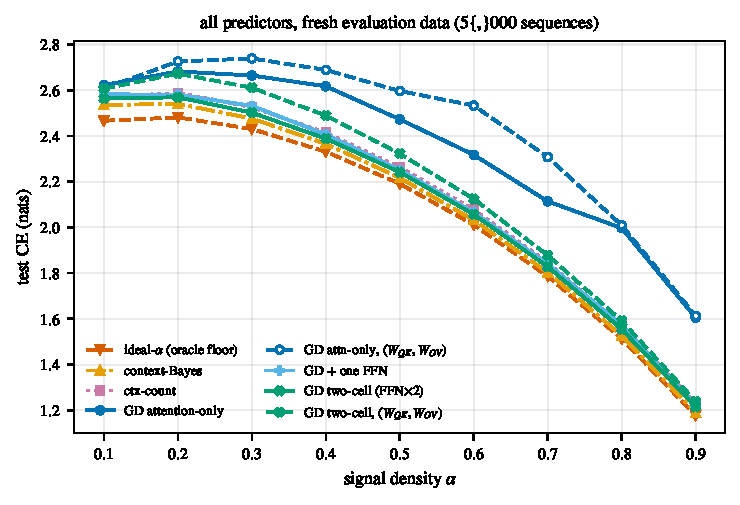
\includegraphics[width=0.78\textwidth]{figures/fig_all_curves.pdf}
\caption{All predictors and model families on one axis (fresh evaluation data).}
\label{fig:all}
\end{figure}

\begin{figure}[h]
\centering
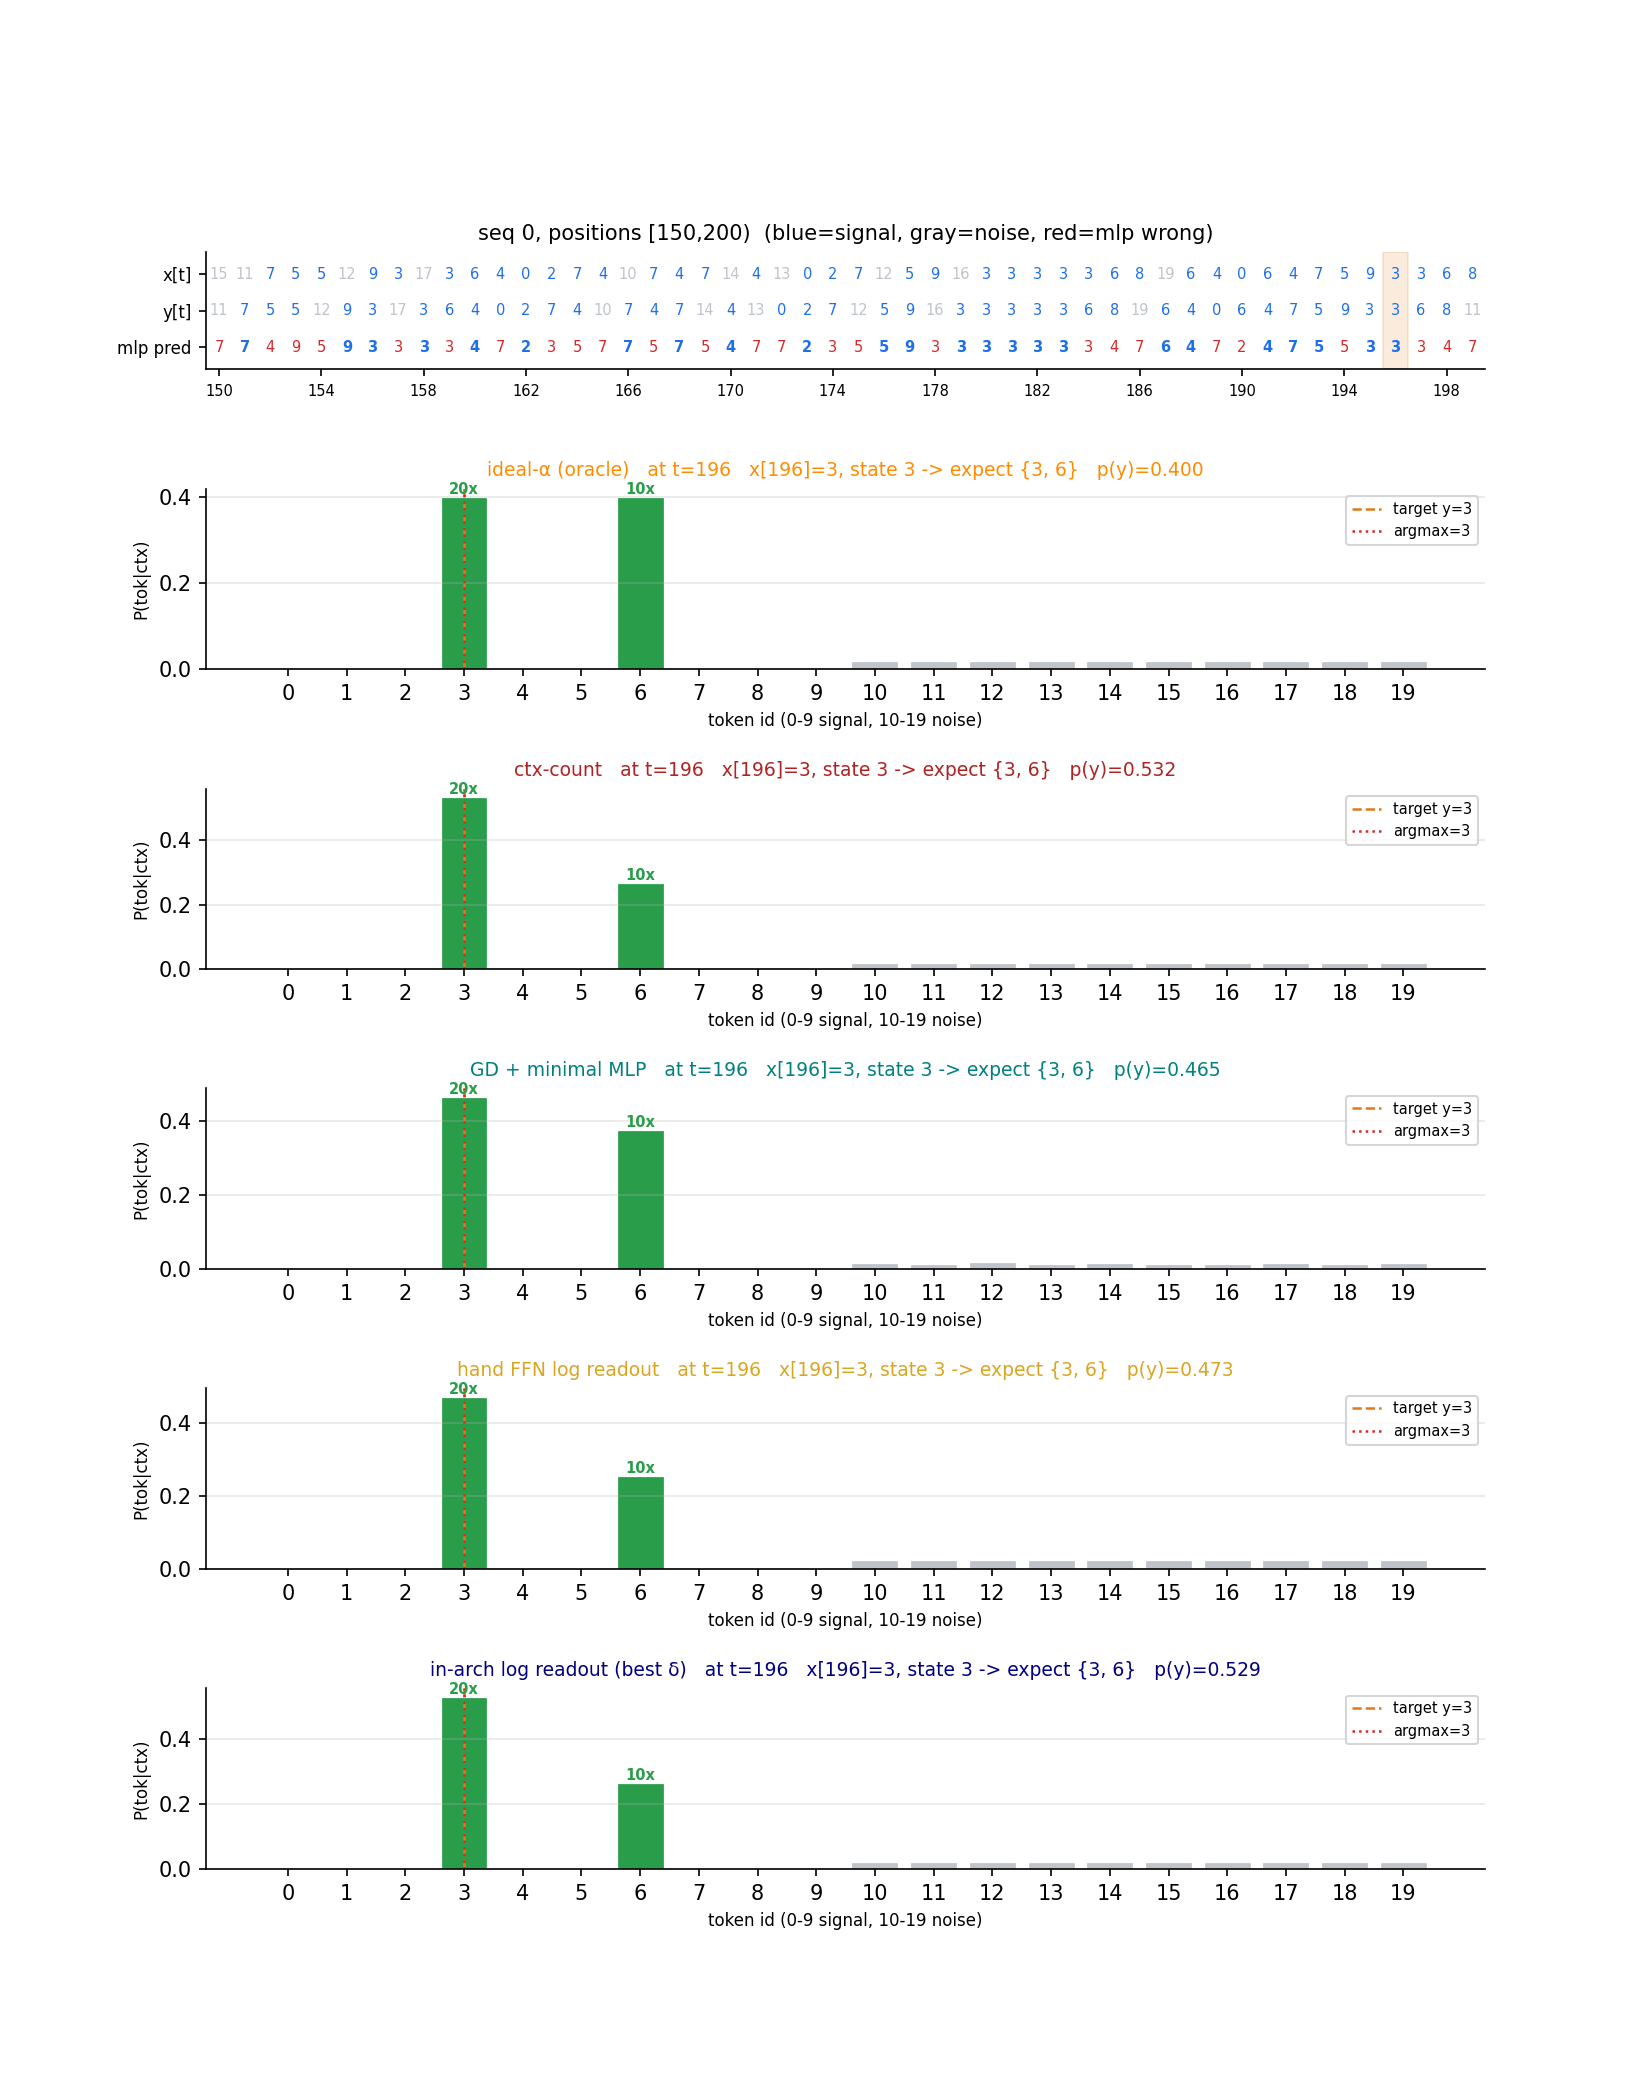
\includegraphics[width=0.9\textwidth]{figures/fig_inspect.png}
\caption{Per-position diagnostic at $\alpha=0.8$ (sequence $0$, focus position
$196$): token strip, the sequence's ground-truth chain, and the predicted
distribution of each predictor alongside the in-context evidence for the queried
state. The trained FFN model places $\approx\alpha/2$ on each observed successor and
the exact floor on noise---the \ctxbayes{} pattern of \S\ref{sec:ffn}.}
\label{fig:inspect}
\end{figure}

\end{document}
